\documentclass[12pt,a4paper]{article}
\usepackage{fancyhdr}
\usepackage{fontspec}
\usepackage{amsmath}
\usepackage{amssymb}
\usepackage{bm}
\usepackage{tikz}
\usepackage{pstricks-add}
\setmainfont{Microsoft YaHei}
\pagestyle{fancy}


\begin{document}

\fancyfoot[C]{by chinasjtu@msn.com }

\newcommand{\nl}{\newline}

\newcommand{\ntinf}{\lim\limits_{n \to \infty}}
\newcommand{\xtinf}{\lim\limits_{x \to \infty}}

\newcommand{\Atinf}{\lim\limits_{A \to \infty}}
\newcommand{\Rtinf}{\lim\limits_{R \to \infty}}

\newcommand{\ntx}[1]{\lim\limits_{n \to #1}}
\newcommand{\xtx}[1]{\lim\limits_{x \to #1}}
\newcommand{\ttx}[1]{\lim\limits_{t \to #1}} 
\newcommand{\ktx}[1]{\lim\limits_{k \to #1}} 
\newcommand{\dxtx}[1]{\lim\limits_{\Delta x \to #1}}

\newcommand{\jfab}{\int_{a}^{b}}
\newcommand{\jf}[2]{\int_{#1}^{#2}}

\newcommand{\nsum}[2]{\sum\limits_{n=#1}^{#2}}
\newcommand{\isum}[2]{\sum\limits_{i=#1}^{#2}}
\newcommand{\ksum}[2]{\sum\limits_{k=#1}^{#2}}

\newcommand{\nsuminf} {\nsum{1}{\infty}}
\newcommand{\ksuminf} {\ksum{1}{\infty}}
\newcommand{\isuminf} {\isum{1}{\infty}}



$\nl$

\begin{center} 第8章 定积分应用  \end{center}




$y=e^{-x}sinx与x轴面积S=\frac{1}{2}\frac{e^\pi+1}{e^\pi-1}$

$Pescartes叶形线x^3+y^3=3axy(a>0)所围成面积$

$化成极坐标系 =\frac{9}{2}a^2 \jf{0}{\frac{\pi}{2}}\frac{sec^2 \theta tg^2 \theta}{(1+tg3\theta)^2}d \theta$


% http://tex.stackexchange.com/questions/224861/folium-of-descartes

\begin{figure}[!ht] 
%\centering 
\psset{algebraic=true,dimen=middle,dotstyle=o,linewidth=0.8pt,arrowsize=3pt 2,arrowinset=0.25,unit=3,plotpoints = 2000} 
\begin{pspicture*}(-1.2,-1.2)(1.2,1.2) 
%\psset{linecolor =black, linewidth = 1.2pt} 

\pscustom[fillstyle = solid, fillcolor =white!25!]{ 
\parametricplot{-0.6}{0}{t/(1 + t^3) | t^2/(1 + t^3)} 
\parametricplot{-100}{-1.5}{t/(1 + t^3) | t^2/(1 + t^3)} } 

\pscustom[fillstyle = solid, fillcolor =black!25! ]{ 
%\parametricplot{0}{5}{3*t/(1 + t^3) | 3*t^2/(1 + t^3)} 
%\parametricplot{5}{200}{3*t/(1 + t^3) | 3*t^2/(1 + t^3)} 
\parametricplot{0}{5}{t/(1 + t^3) | t^2/(1 + t^3)} 
\parametricplot{5}{10}{t/(1 + t^3) | t^2/(1 + t^3)} 

\closepath } 

%\psline[linewidth = 0.4pt, linecolor = black](-2.5; 45)(2.5 ; 45) 
\psline[linewidth = 0.4pt, linecolor = black](-0.9,0.5)(0.6,-1) 
\psaxes[linecolor=black,xAxis=true,yAxis=true,labels=none,ticks=none]{->}(0,0)(-1,-1)(1,1) 
\end{pspicture*} 
\end{figure}



$=\frac{3}{2}a^2$

$x=\frac{3at}{1+t^2},y=\frac{3at^2}{1+t^2}$

$\nl$
$抛物线沿0x轴滚动,焦点画出悬链线$

$\nl$

$示例:求椭圆\frac{x^2}{a^2}+\frac{y^2}{b^2}=1及平面z=\frac{c}{a}x,y=0所围立体体积$

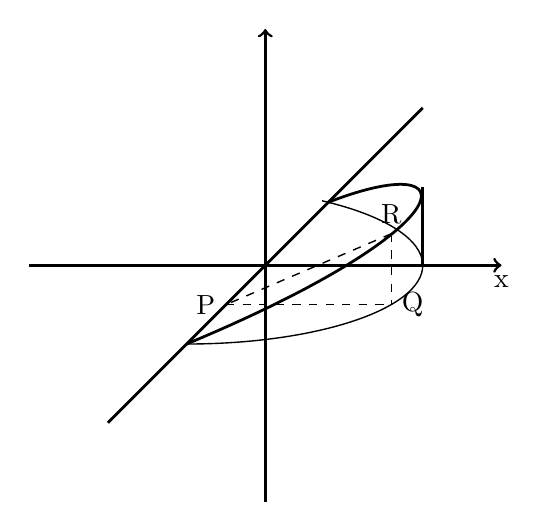
\begin{tikzpicture}[domain=1:5,line width=1pt]
\draw[->] (-3,0) -- (3,0);
\draw[->] (0,-3) -- (0,3);
\draw (-2,-2) -- (2,2);
\draw (2,0) -- (2,1);

\draw[style=dashed, line width=0.5 pt] (-0.5,-0.5) -- (1.6,-0.5);
\draw[style=dashed, line width=0.5 pt] (1.6,0.4) -- (1.6,-0.5);
\draw[style=dashed, line width=0.5 pt] (1.6,0.4) -- (-0.5,-0.5);

\node [left] at (-0.5,-0.5) {P}; 
\node [right] at (1.6,-0.5) {Q}; 
\node [above] at (1.6,0.4) {R}; 

%\draw[line  width=0.5 pt] (-1,-1) arc (270:405:3 and 1);
\draw[line  width=0.5 pt] (-1,-1) arc (270:415:3 and 1);

\draw(-1,-1)..controls (2.6,0.5) and (2.6,1.5)..(0.8,0.8);

\node [below] at (3,0) {x};        
\end{tikzpicture}


$对y\in[-b,b]过y作垂直于y轴平面截立体的截面为直角三角形PRQ,且有PQ=x=a\sqrt{1-\frac{y^2}{b^2}},QR=c\sqrt{1-\frac{y^2}{b^2}}$

$从而截面积函数为S(y)=\frac{1}{2}ac(1-\frac{y^2}{b^2})$

$V=\jf{-b}{b}dV=\jf{-b}{b}\frac{1}{2}ac(1-\frac{y^2}{b^2})dy=\frac{2}{3}abc$

$\nl$
$求Viviand体,由x^2+y^2+z^2=a^2,x^2+y^2=ax(a>0)围成体积$

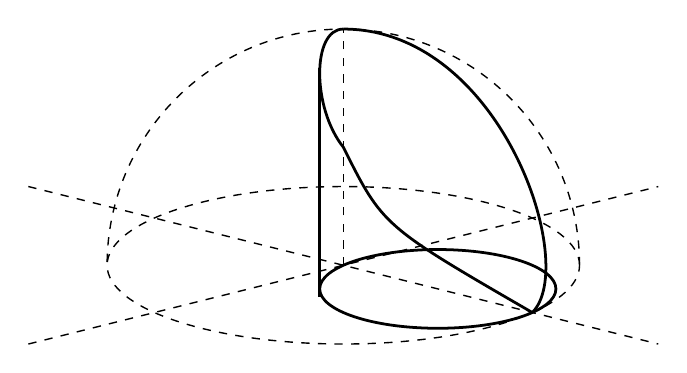
\begin{tikzpicture}[domain=1:5,line width=1pt]
\draw[style=dashed, line width=0.5 pt] (-4,-1) -- (4,1);
\draw[style=dashed, line width=0.5 pt] (-4,1) -- (4,-1);
\draw[style=dashed, line width=0.5 pt] (0,0) -- (0,3);

\draw[style=dashed, line width=0.5 pt]  (0,0)  ellipse  (3 and 1);
\draw[style=dashed, line width=0.5 pt]  (3,0)  arc  (0:180:3);

\draw(2.4,-0.6)..controls (3,0) and (2,3)..(0,3);

\draw  (2.4,-0.6)..controls (0.5,0.5)..(0,1.5)..controls (-0.4,2) and (-0.4,3) .. (0,3);

\draw (1.2,-0.3)  ellipse  (1.5 and 0.5);
\draw (-0.3,-0.4) -- (-0.3,2.5);
\end{tikzpicture}

$\nl$
$物理应用(示例规范)$

$从高为H,半径为R的圆锥桶中吸出密度为M的液体的功$

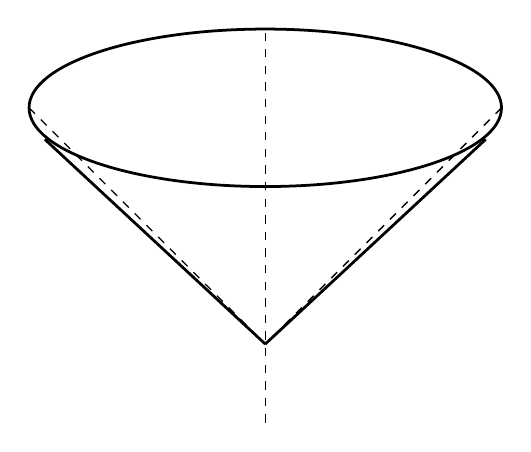
\begin{tikzpicture}[domain=1:5,line width=1pt]
\draw[style=dashed, line width=0.5 pt] (0,-4) -- (0,1);

\draw[line width=1 pt]  (0,0)  ellipse  (3 and 1);
\draw[style=dashed, line width=0.5 pt] (3,0) -- (0,-3);
\draw[style=dashed, line width=0.5 pt] (-3,0) -- (0,-3);

\draw[line width=1 pt] (2.8,-0.4) -- (0,-3);
\draw[line width=1 pt] (-2.8,-0.4) -- (0,-3);

\end{tikzpicture}

$解:取坐标如图,基本区间为0 \le x \le H$

$在[0,H]上任取x,x+dx,则从桶内抽出位于[x,x+dx]层上液体所做功为$

$dW=\pi r^2 dx M (H-x),r=\frac{R}{H}x$

$W=\frac{1}{12}M\pi R^2H^2$

$\nl$

$定理1,设弧\overset{\frown} {AB},x=x(t),y=y(t),在[\alpha,\beta]连续,线密度为\lambda (t) \in c[\alpha,\beta]$

$则\overset{\frown} {AB}重心坐标\overline x=\frac{\jf{\alpha}{\beta}x(t)\lambda(t)ds}{\jf{\alpha}{\beta}\lambda(t)ds},\overline y=\frac{\jf{\alpha}{\beta}y(t)\lambda(t)ds}{\jf{\alpha}{\beta}\lambda(t)ds}$

$其中ds=\sqrt{x^2(t)+y^2(t)}dt为弧微分$

$\nl$

$定理2:设质量均匀平面图形D,y=f(x) \ge 0, x=a x=b及x轴$

$则D质心为\overset{\frown} {x}=\frac{\jf{a}{b}xydx}{\jf{a}{b}ydx},\overset{\frown} {y}=\frac{\frac{1}{2}\jf{a}{b}y^2dx}{\jf{a}{b}ydx}$

$Guldin定理$

$(1)平面弧,\overset{\frown} {AB}长度为l,绕定轴旋转(\overset{\frown} {AB}不穿过轴)$

$其质心到转轴距离为\eta,则有S=2\pi \eta l,其中S为旋转曲面表面积$

$(2)平面图形D面积S,绕定轴旋转(D不穿过轴)其质心到轴距离为\eta ,则有V=2\pi \eta S,其中V为旋转体体积$

$\nl$

$例:求质心绕x轴旋转,旋转体体积$

$V=2\pi \eta \pi R^2-2\pi \eta \pi r^2$

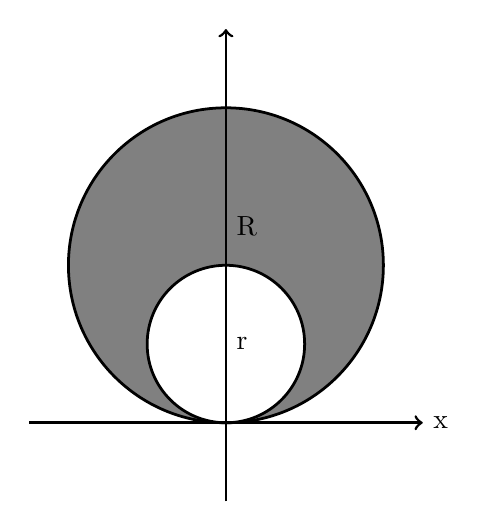
\begin{tikzpicture}[domain=1:5,line width=1pt]
\draw[fill=gray] (0,2) circle (2);
\draw[fill=white] (0,1) circle (1);
\draw[->] (0,-1) -- (0,5);
\draw[->] (-2.5,0) -- (2.5,0);
\node[right] at (2.5,0) {x};
\node[right] at (0,1) {r};
\node[right] at (0,2.5) {R};
\end{tikzpicture}

\end{document}

